%%%%%%%%%%%%%%%%%%%%%%%%%%%%%%%%%%%%%%%%%
% Medium Length Professional CV
% LaTeX Template
% Version 2.0 (8/5/13)
%
% This template has been downloaded from:
% http://www.LaTeXTemplates.com
%
% Original author:
% Rishi Shah 
%
% Important note:
% This template requires the resume.cls file to be in the same directory as the
% .tex file. The resume.cls file provides the resume style used for structuring the
% document.
%
%%%%%%%%%%%%%%%%%%%%%%%%%%%%%%%%%%%%%%%%%

%----------------------------------------------------------------------------------------
%	PACKAGES AND OTHER DOCUMENT CONFIGURATIONS
%----------------------------------------------------------------------------------------

\documentclass{resume} % Use the custom resume.cls style
\usepackage{hyperref}
\usepackage{tikz}
\usepackage{polski}
\usepackage[utf8]{inputenc}
\usepackage[left=0.75in,top=0.2in,right=0.75in,bottom=0.2in]{geometry} % Document margins
\newcommand{\tab}[1]{\hspace{.2667\textwidth}\rlap{#1}}
\newcommand{\itab}[1]{\hspace{0em}\rlap{#1}}

\name{Jakub Płotnikowski}

\address{\small \url{https://www.linkedin.com/in/jakub-plotnikowski}
\\ \small \url{https://github.com/jakubowiczish}}
\address{(+48) 668 793 372 \\ plotnikowskijakub@gmail.com \\ Kraków}

\begin{document}

\begin{tikzpicture}[remember picture, overlay]
  \node [anchor=north east, inner xsep=40pt, inner ysep=20pt]  at (current page.north east)
     {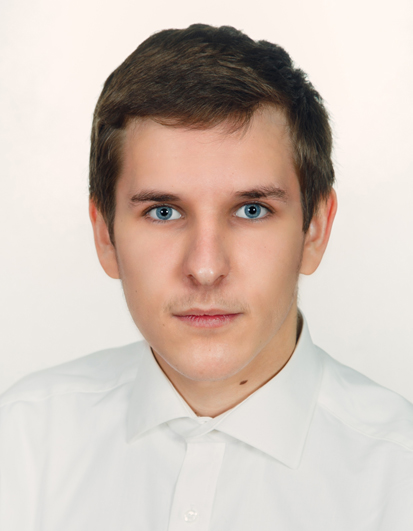
\includegraphics[height=3cm]{PICTURE.jpg}};
\end{tikzpicture}

%----------------------------------------------------------------------------------------
%	WORK EXPERIENCE SECTION
%----------------------------------------------------------------------------------------
\begin{rSection}
{Work Experience}

\begin{rSubsection}
{Grand Parade part of William Hill}
{Jul. 2020 - now}
{Junior Software Developer}

Member of a team that was responsible for:

\begin{itemize}

\item{Development of backend microservices responsible for various betting mechanisms as well as wallet and account management}

\end{itemize}
\end{rSubsection}

\begin{rSubsection}
{Softnet Systemy Bankowe}
{Jul. 2019 - Jun. 2020}
{Junior Software Developer}

\begin{itemize}

\item{Development of mobile application for cooperative banking and backend application that is an implementation of PolishAPI}

\item{Maintenance and development of new features for application designed for individual banking clients.}

\end{itemize}
\end{rSubsection}

\end{rSection}

%----------------------------------------------------------------------------------------
%	EDUCATION SECTION
%----------------------------------------------------------------------------------------

\begin{rSection}{Education}

{\bf AGH University of Science and Technology} \hfill {Oct. 2017 - now}
\\ Faculty of Computer Science, Electronics and Telecommunications
\\ Computer Science

\end{rSection}

%--------------------------------------------------------------------------------
%    SKILLS
%--------------------------------------------------------------------------------

\begin{rSection}{Skills}
\begin{itemize}
 \setlength\itemsep{-0.5em}
\item Programming in object-oriented paradigm
\item Main technologies used: Java, Git, Spring, Spring Boot, Hibernate, Android, JUnit, Mockito, PostgreSQL, PL/SQL, Liquibase, Maven, Gradle, Docker, Scala
\item Knowledge of RESTful API, Clean Code rules and Design Patterns
\item Knowledge of algorithms and data structures
\item Soft skilled, hard-working, ambitious, willing to learn logical thinker
\item English – C1, FCE
\end{itemize}
\end{rSection}


%--------------------------------------------------------------------------------
%    PROJECTS
%--------------------------------------------------------------------------------

\begin{rSection}{Projects}
\begin{itemize}
 \setlength\itemsep{0em}

\item \textbf{Master-Diet} Web application written in Spring Boot and React for managing diet with some gamification features.

\item \textbf{DiaBeFriend} - Android application for people with diabetes, written in Java.
It provides user with features that
help manage everyday life with this illness e.g. tracking sugar intake after meals, searching for food with appropriate nutritional data in existing database of products.

 More info and source code on: \url{https://github.com/jakubowiczish/DiaBeFriend}

\item \textbf{AirPollution} - Java console application that provides user with various information about air quality in Poland.

\item \textbf{Conferences} – The objective of this project was to create the entire database that will manage the organization
of various conferences - it required designing the database schema, ensuring database data integrity and
implementing triggers, views, procedures, functions using SQL as well as data generator.

\item \textbf{BibTeX parser} - Java console application that allows user to search and manipulate data that given BibTeX file
contains.
\end{itemize}
\end{rSection}

%--------------------------------------------------------------------------------
%    INTERESTS
%--------------------------------------------------------------------------------

\begin{rSection}{Interests}
Meeting new people, electronic music, middle-distance running, astronomy, traveling, board games, computer games
\end{rSection}

%--------------------------------------------------------------------------------
%    PERSONAL DATA PROCESSING AGREEMENT
%--------------------------------------------------------------------------------

\vfill
\footnotesize „I agree to the processing of personal data provided in this document for realising the recruitment process
pursuant to the Personal Data Protection Act of 10 May 2018 (Journal of Laws 2018, item 1000) and in
agreement with Regulation (EU) 2016/679 of the European Parliament and of the Council of 27 April 2016 on
the protection of natural persons with regard to the processing of personal data and on the free movement of
such data, and repealing Directive 95/46/EC (General Data Protection Regulation)”.

\end{document}